\documentclass[14pt]{extbook}
\usepackage{multicol, enumerate, enumitem, hyperref, color, soul, setspace, parskip, fancyhdr} %General Packages
\usepackage{amssymb, amsthm, amsmath, bbm, latexsym, units, mathtools} %Math Packages
\everymath{\displaystyle} %All math in Display Style
% Packages with additional options
\usepackage[headsep=0.5cm,headheight=12pt, left=1 in,right= 1 in,top= 1 in,bottom= 1 in]{geometry}
\usepackage[usenames,dvipsnames]{xcolor}
\usepackage{dashrule}  % Package to use the command below to create lines between items
\newcommand{\litem}[1]{\item#1\hspace*{-1cm}\rule{\textwidth}{0.4pt}}
\pagestyle{fancy}
\lhead{Progress Quiz 8}
\chead{}
\rhead{Version A}
\lfoot{4553-3922}
\cfoot{}
\rfoot{Fall 2020}
\begin{document}

\begin{enumerate}
\litem{
Write the equation of the line in the graph below in Standard form $Ax+By=C$. Then, choose the intervals that contain $A, B, \text{ and } C$.
\begin{center}
    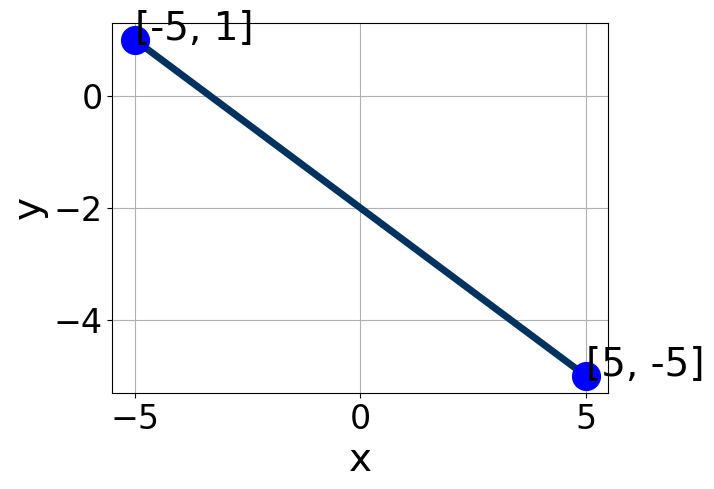
\includegraphics[width=0.5\textwidth]{../Figures/linearGraphToStandardA.png}
\end{center}
\begin{enumerate}[label=\Alph*.]
\item \( A \in [1.1, 6.8], \hspace{3mm} B \in [4.4, 5.7], \text{ and } \hspace{3mm} C \in [-29, -21] \)
\item \( A \in [-1.5, 1.1], \hspace{3mm} B \in [0.7, 4.2], \text{ and } \hspace{3mm} C \in [-5, -4] \)
\item \( A \in [1.1, 6.8], \hspace{3mm} B \in [-6.3, -1.8], \text{ and } \hspace{3mm} C \in [25, 30] \)
\item \( A \in [-4.2, -0.7], \hspace{3mm} B \in [-6.3, -1.8], \text{ and } \hspace{3mm} C \in [25, 30] \)
\item \( A \in [-1.5, 1.1], \hspace{3mm} B \in [-1.4, 0.7], \text{ and } \hspace{3mm} C \in [5, 8] \)

\end{enumerate} }
\litem{
Solve the equation below. Then, choose the interval that contains the solution.\[ -17(6x -18) = -13(9x + 5) \]\begin{enumerate}[label=\Alph*.]
\item \( x \in [-27.73, -23.73] \)
\item \( x \in [-20.07, -15.07] \)
\item \( x \in [-1.9, 3.1] \)
\item \( x \in [15.07, 18.07] \)
\item \( \text{There are no real solutions.} \)

\end{enumerate} }
\litem{
Solve the linear equation below. Then, choose the interval that contains the solution.\[ \frac{-7x -9}{4} - \frac{-4x -9}{2} = \frac{5x -3}{8} \]\begin{enumerate}[label=\Alph*.]
\item \( x \in [6.6, 7.2] \)
\item \( x \in [-18.5, -15.4] \)
\item \( x \in [-1.3, 0.4] \)
\item \( x \in [7.9, 9] \)
\item \( \text{There are no real solutions.} \)

\end{enumerate} }
\litem{
Find the equation of the line described below. Write the linear equation as $ y=mx+b $ and choose the intervals that contain $m$ and $b$.\[ \text{Perpendicular to } 5 x - 3 y = 3 \text{ and passing through the point } (-7, -3). \]\begin{enumerate}[label=\Alph*.]
\item \( m \in [-1.6, 0.4] \hspace*{3mm} b \in [-12.2, -4.2] \)
\item \( m \in [-1.6, 0.4] \hspace*{3mm} b \in [5.2, 12.2] \)
\item \( m \in [-0.4, 2.6] \hspace*{3mm} b \in [0.2, 2.2] \)
\item \( m \in [-1.6, 0.4] \hspace*{3mm} b \in [3, 7] \)
\item \( m \in [-2.67, -0.67] \hspace*{3mm} b \in [-12.2, -4.2] \)

\end{enumerate} }
\litem{
First, find the equation of the line containing the two points below. Then, write the equation as $ y=mx+b $ and choose the intervals that contain $m$ and $b$.\[ (-8, 10) \text{ and } (3, -6) \]\begin{enumerate}[label=\Alph*.]
\item \( m \in [-1.96, -0.4] \hspace*{3mm} b \in [0.94, 2.54] \)
\item \( m \in [-1.96, -0.4] \hspace*{3mm} b \in [-9.18, -7.8] \)
\item \( m \in [1.03, 1.61] \hspace*{3mm} b \in [-10.99, -9.32] \)
\item \( m \in [-1.96, -0.4] \hspace*{3mm} b \in [17.79, 19] \)
\item \( m \in [-1.96, -0.4] \hspace*{3mm} b \in [-2.83, -0.36] \)

\end{enumerate} }
\litem{
Solve the linear equation below. Then, choose the interval that contains the solution.\[ \frac{5x + 4}{5} - \frac{7x -5}{4} = \frac{-3x -5}{3} \]\begin{enumerate}[label=\Alph*.]
\item \( x \in [-15.2, -14.3] \)
\item \( x \in [-56.2, -55.7] \)
\item \( x \in [-7.1, -4.6] \)
\item \( x \in [-3.9, -2.2] \)
\item \( \text{There are no real solutions.} \)

\end{enumerate} }
\litem{
Find the equation of the line described below. Write the linear equation as $ y=mx+b $ and choose the intervals that contain $m$ and $b$.\[ \text{Perpendicular to } 8 x - 7 y = 15 \text{ and passing through the point } (-8, 6). \]\begin{enumerate}[label=\Alph*.]
\item \( m \in [-1.1, -0.61] \hspace*{3mm} b \in [0.86, 1.16] \)
\item \( m \in [-1.37, -0.95] \hspace*{3mm} b \in [-2.09, -0.58] \)
\item \( m \in [-1.1, -0.61] \hspace*{3mm} b \in [13.5, 14.51] \)
\item \( m \in [-1.1, -0.61] \hspace*{3mm} b \in [-2.09, -0.58] \)
\item \( m \in [0.76, 1.11] \hspace*{3mm} b \in [12.58, 13.02] \)

\end{enumerate} }
\litem{
Solve the equation below. Then, choose the interval that contains the solution.\[ -12(6x + 14) = -8(-18x -5) \]\begin{enumerate}[label=\Alph*.]
\item \( x \in [-0.7, -0.4] \)
\item \( x \in [1.56, 2.02] \)
\item \( x \in [0.31, 0.64] \)
\item \( x \in [-1.27, -0.88] \)
\item \( \text{There are no real solutions.} \)

\end{enumerate} }
\litem{
First, find the equation of the line containing the two points below. Then, write the equation as $ y=mx+b $ and choose the intervals that contain $m$ and $b$.\[ (-3, -11) \text{ and } (-7, -9) \]\begin{enumerate}[label=\Alph*.]
\item \( m \in [-0.9, -0.3] \hspace*{3mm} b \in [12.2, 15.9] \)
\item \( m \in [-0.9, -0.3] \hspace*{3mm} b \in [-9.9, -7.3] \)
\item \( m \in [-0.9, -0.3] \hspace*{3mm} b \in [-2.8, -0.2] \)
\item \( m \in [-0.9, -0.3] \hspace*{3mm} b \in [-14.3, -10.7] \)
\item \( m \in [-0.4, 2.4] \hspace*{3mm} b \in [-7.5, -2.5] \)

\end{enumerate} }
\litem{
Write the equation of the line in the graph below in Standard form $Ax+By=C$. Then, choose the intervals that contain $A, B, \text{ and } C$.
\begin{center}
    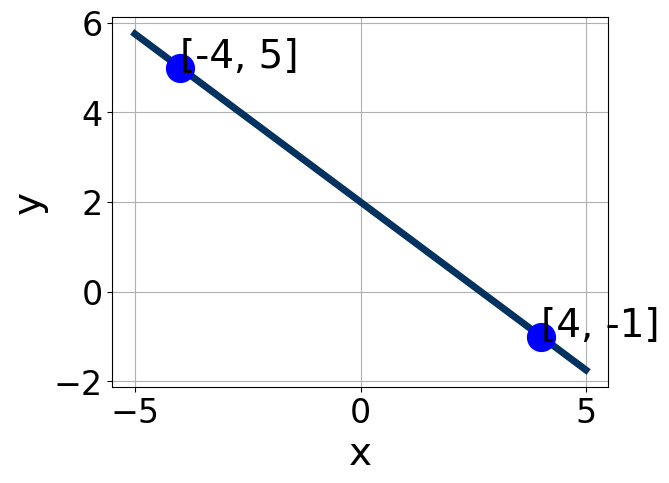
\includegraphics[width=0.5\textwidth]{../Figures/linearGraphToStandardCopyA.png}
\end{center}
\begin{enumerate}[label=\Alph*.]
\item \( A \in [2.6, 4.1], \hspace{3mm} B \in [-5, -3], \text{ and } \hspace{3mm} C \in [9, 16] \)
\item \( A \in [-1.6, 2.3], \hspace{3mm} B \in [0, 2], \text{ and } \hspace{3mm} C \in [-8, 1] \)
\item \( A \in [-1.6, 2.3], \hspace{3mm} B \in [-1, 0], \text{ and } \hspace{3mm} C \in [1, 7] \)
\item \( A \in [-3.2, -2.8], \hspace{3mm} B \in [3, 6], \text{ and } \hspace{3mm} C \in [-12, -10] \)
\item \( A \in [2.6, 4.1], \hspace{3mm} B \in [3, 6], \text{ and } \hspace{3mm} C \in [-12, -10] \)

\end{enumerate} }
\end{enumerate}

\end{document}